\documentclass[12pt]{article}
\usepackage{amsmath, amssymb, amsthm}
\usepackage{setspace}
\usepackage{graphicx}
\usepackage{mathtools}
\usepackage{float}
\usepackage{algorithm}
\usepackage{algpseudocode}
\usepackage{listings}
\usepackage{enumitem}
\usepackage[russian]{babel} 

\usepackage[margin=1in]{geometry}

\begin{document}

\title{\textbf{Марковская цепь как случайный процесс}}
\author{Выполнила Карина Лирисман, группа Б01-008}
\date{}

\maketitle

\section{Введение}

\textit{Марковский процесс} - это стохастический процесс, в котором вероятность перехода состояний зависит только от текущего состояния и не зависит от предыдущих состояний (т.е. обладает свойством Маркова). Марковский процесс удобен для моделирования многих систем, таких как финансовые рынки, экономические и социологические процессы, погода и другие случайные явления.

\subsection{Марковская цепь}

\textit{Марковская цепь} - это стохастический процесс, который определяется из состояний и переходов между этими состояниями. 

Формально, мы можем определить марковскую цепь $\{X_n\}$ на конечном множестве состояний $S = \{s_1, s_2, ..., s_n\}$ следующим образом. Если $X_n$ находится в состоянии $s_i$, то вероятность перейти в состояние $s_j$ на следующем шаге (т.е. в момент времени $n+1$) обозначим $P_{ij}$, где $i,j \in S$ и $\sum_{j}P_{ij}=1$.

Марковская цепь является временно \textit{однородной}, если матрица переходных вероятностей $P_{ij}$ не меняется со временем. Если матрица переходных вероятностей зависит от времени, то мы говорим, что марковская цепь \textit{нестационарна}.

\section{Случайный процесс}

\textit{Случайный процесс$^1$} - это семейство случайных переменных $\{X_t : t \in T\}$ на общем вероятностном пространстве. Для каждого фиксированного $t \in T$, $X_t$ - это случайная переменная. \textit{Случайный процесс в узком смыслe} - это коллекция случайных величин, определенных на одном и том же вероятностном пространстве, и индексированных некоторым параметром. Например, если мы рассматриваем случайный процесс, описывающий движение частицы в жидкости, то каждая случайная величина может соответствовать координате частицы в разные моменты времени. Таким образом, случайный процесс позволяет нам моделировать эволюцию случайных величин во времени.

Теперь введем понятие \textit{Колмогоровского пространства}: но представляет собой математическую конструкцию, которая позволяет определить вероятностное пространство для любого случайного процесса.

Формально, \textit{колмогоровское пространство$^1$} определяется следующим образом. Пусть $T$ - некоторое параметризующее множество, $S$ - множество состояний, и для каждого $t \in T$ задано вероятностное пространство $(S_t, \mathcal{F}_t, P_t)$, где $S_t$ - множество состояний на момент времени $t$, $\mathcal{F}_t$ - $\sigma$-алгебра событий на $S_t$, а $P_t$ - вероятностная мера на $(S_t, \mathcal{F}_t)$. Тогда колмогоровское пространство с функциями определяется как пространство функций $X: T \to S$, для которых каждая компонента $X_t$ является случайной величиной на $(S_t, \mathcal{F}_t, P_t)$.

Наконец, введем понятие \textit{сигма-алгебры}. \textit{Сигма-алгебра$^1$} - это коллекция подмножеств некоторого множества, которая обладает рядом свойств, например, она замкнута относительно операций объединения, пересечения и дополнения. В контексте вероятностной теории, сигма-алгебра используется для описания множества событий, которые могут возникнуть в результате случайного эксперимента. Сигма-алгебра $\sigma(X_t)$, порожденная случайной величиной $X_t$, состоит из всех событий, которые можно выразить через $X_t$. Таким образом, $\sigma(X_t)$ содержит все информацию о состоянии процесса $X$ в момент времени $t$.

Колмогоровское пространство с функциями и связанная с ним сигма-алгебра $\sigma(X_t)$ являются важными концепциями в теории вероятностей, так как они позволяют определить вероятностное пространство для любого случайного процесса и задать информационную структуру процесса. 

Случайный процесс также можно рассматривать как индексированный набор случайных величин в некоторый момент времени. Если множество временных меток $T$ является интервалом времени, то случайный процесс называется непрерывным во времени. Если $T$ конечен или состоит из дискретных меток времени, то случайный процесс называется дискретным во времени.

В данном случае переходы системы из одного в другое состояние возможно в строго определенные моменты времени ${t_0}$, ${t_1}$, …, ${t_n}$ , а случайный
процесс $X(t_i)$ в промежутках между указанными моментами времени сохраняет свое состояние (см рис.\ref{figure1}). Такие процессы встречаются при машинной обработке информации в цифровых ЭВМ. 

\begin{figure}[!ht]
\begin{center}
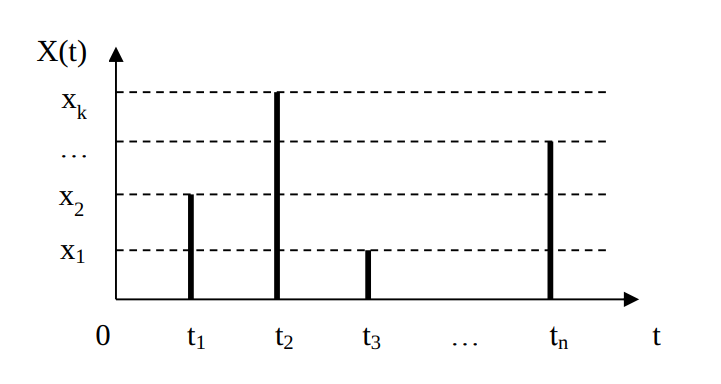
\includegraphics[scale=0.5]{1_pic.png}\caption{}\label{figure1}
\end{center}
\end{figure}

Случайный процесс называется \textit{дискретным Марковским процессом$^2$}, если его состояния можно пронумеровать и переход из одного в другое состояния происходит скачком (см рис.\ref{figure2})

\begin{figure}[!ht]
\begin{center}
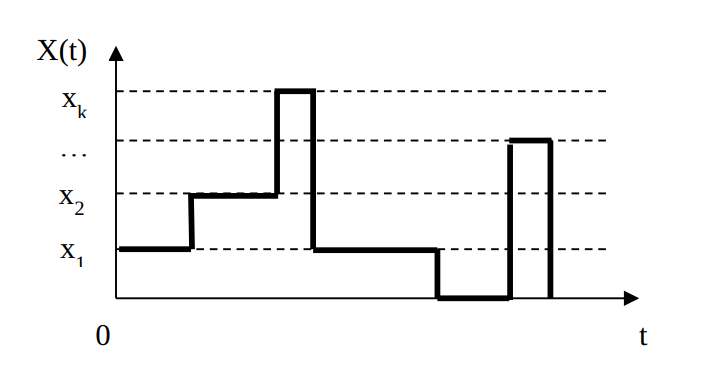
\includegraphics[scale=0.5]{2_pic.png}\caption{}\label{figure2}
\end{center}
\end{figure}

В этом случае случайный процесс $X(t)$ принимает дискретные значения $х_i$, i = 1 … n, время t изменяется непрерывно.

\section{Теорема Колмогорова}

Теорема Колмогорова утверждает, что для любой временно однородной марковской цепи с конечным числом состояний существует минимальное неотрицательное целое число n, такое что $P_{ij}^{(n)} > 0$ для всех $i,j \in S$. То есть, начиная с некоторого момента времени, вероятность перехода между любой парой состояний становится положительной.

Теорема Колмогорова устанавливает \textit{свойство стационарности$^2$} марковских цепей. Она гласит, что если марковская цепь удовлетворяет условию эргодичности, то существует единственное стационарное распределение вероятностей в этой цепи, которое не зависит от начального состояния.

Теперь, когда определены основные термины, переходим к Марковской цепи.

\section{Цепь Маркова как случайный процесс}

\textit{Марковская цепь$^3$} – это последовательность случайных событий, где вероятность следующего события зависит только от текущего. В этом смысле марковские цепи являются случайным процессом. В отличие от других случайных процессов, марковские цепи не имеют памяти, то есть не сохраняют информацию о предыдущих событиях.

Особый интерес представляют марковские процессы с конечным числом состояний, которые называются цепями Маркова с дискретным временем. Для таких процессов можно вычислить стационарные распределения и вероятности переходов между состояниями.

\subsection{Марковский случайный процесс с дискретными состояниями и дискретным временем (цепь Маркова)}

\textit{Дискретным Марковским процессом с дискретными состояниями и дискретным временем$^3$} называют процесс, в котором возможные состояния системы $S_1$, $S_2$, … , $S_n$ можно перечислить (пронумеровать), а сам процесс перехода системы из одного в другое состояние происходит в фиксированные моменты времени $t_1$, $t_2$, $t_3$, … $t_n$. В промежутках между этими моментами времени система сохраняет свое состояние.

При любом шаге перехода системы события переходов образуют полную группу и несовместны, так как система может находиться лишь в одном из состояний, а не в двух и более сразу. При этом рассматриваются
все возможные состояния системы. 

Если каждое состояние системы в k-й момент времени свяжем с вероятностью, то получим вероятности состояний $P(k)_1$, $P(k)_2$, $P(k)_3$, … , $P(k)_n$. Для
любого момента времени $P(k)_1$ + $P(k)_2$ +,…, + $P(k)_n$ = 1

Для любого момента времени $t_1$, $t_2$, $t_3$,…, $t_k$, существуют вероятности перехода системы из любого состояния в любое другое $P_{ij}(k)$ (i, j = 1, 2, , n). Их
называют вероятностями перехода или переходными вероятностями. Эти вероятности отличны от нуля, если система переходит из одного состояния в
другое, и равны нулю, если на данном шаге система остается в прежнем состоянии. 

Если вероятности перехода не зависят от номера шага (момента времени) и не изменяются от шага к шагу, то такой Марковский процесс называют однородным. В противном случае Марковский процесс называют неоднородным.

Вероятностная картина возможных состояний системы и ее переходов может быть задана матрицей Р, элементами которой являются переходные
вероятности: 

\begin{center}

$ P(k)= \begin{bmatrix}
		\ p(k)_{11}& \ p(k)_{12}...& \ p(k)_{1n}\\
		\ p(k)_{21}& \ p(k)_{22}...& \ p(k)_{2n}\\
		\ p(k)_{n1}& \ p(k)_{n2}...& \ p(k)_{nn}\\
		\end{bmatrix}
$
\end{center}

Матрица переходных вероятностей обладает следующими свойствами:
\begin{enumerate}
\item[•] cумма вероятностей, стоящих в каждой строке матрицы равна единице
\item[•] на главной диагонали матрицы стоят вероятности того, что система не выйдет из состояния $S_i$ а останется в нем
\item[•] если переходная вероятность $P_{ij}(k)$ = 0, то это означает, что на данном шаге система не может перейти из состояния $S_i$, в состояние $S_j$.
\end{enumerate}

Имея размеченный граф состояний или матрицу переходных вероятностей и, зная начальное состояние системы, можно найти все возможные вероятности состояний системы для любого момента времени. Для этого используют следующие уравнения:
\begin{enumerate}
\item[-] для однородного Марковского процесса:
\begin{center}
$p(k)_j = \sum_{i=1}^n p_i (k-1)  p_{ij} , j = 1, 2, ... , n$
\end{center}
\item[-] для неоднородного Марковского процесса:
\begin{center}
$p(k)_j = \sum_{i=1}^n p_i (k-1)  p(k)_{ij} , j = 1, 2, ... , n$
\end{center}
\end{enumerate}

\section{Литература}

\begin{enumerate}

\item Ширяев А. Н. Ш64 Вероятность. В 2-х кн. –– 3-е изд., перераб. и доп. ––М.: МЦНМО, 2004. ISBN 5-94057-036-4 Кн. 2. –– 408 с. –– ISBN 5-94057-106-9

\item Булинский А. В., Ширяев А. Н. Теория случайных процессов. — М.: ФИЗМАТЛИТ, 2005. - 408 с. - ISBN 5-9221-0335-0.

\item Статистика случайных процессов (нелинейная фильтрация и смежные вопросы), Лицер Р.Ш., Ширяев А.Н., Главная редакция физико-математической литературы изд-ва "Наука" 1974.

\end{enumerate}

\end{document}